\documentclass[a4paper]{article}
\usepackage[top = 30mm, bottom = 20mm, inner = 30mm, outer = 30mm]{geometry}

\usepackage{graphicx}
\usepackage{float}
\usepackage[english]{babel}
\usepackage[round]{natbib}
\bibliographystyle{abbrvnat}
\bibliographystyle{plainnat}
\usepackage{subcaption}

\usepackage[hidelinks]{hyperref}

\usepackage{multicol}

\usepackage{titlesec}
\titleformat{\section}
{\normalfont\fontsize{11}{13}\bfseries}{\thesection}{1em}{}

\renewcommand{\figurename}{Fig.}
\renewcommand{\thefigure}{S\arabic{figure}}
\renewcommand{\tablename}{Tab.}
\renewcommand{\thetable}{S\arabic{table}}

\renewcommand*{\contentsname}{Table of Contents}

\usepackage{xr}
\externaldocument{OnOffRivers_0_Paper}
\externaldocument{OnOffRivers_OSM_2_Sites}
\externaldocument{OnOffRivers_OSM_3_Petrography}


%opening
\title{Online Supplemental Material (OSM) 1: Supplementary Figures and Tables}
%\author{Dirk Seidensticker}

\begin{document}

\maketitle

\begin{figure}[H]
	\centering
	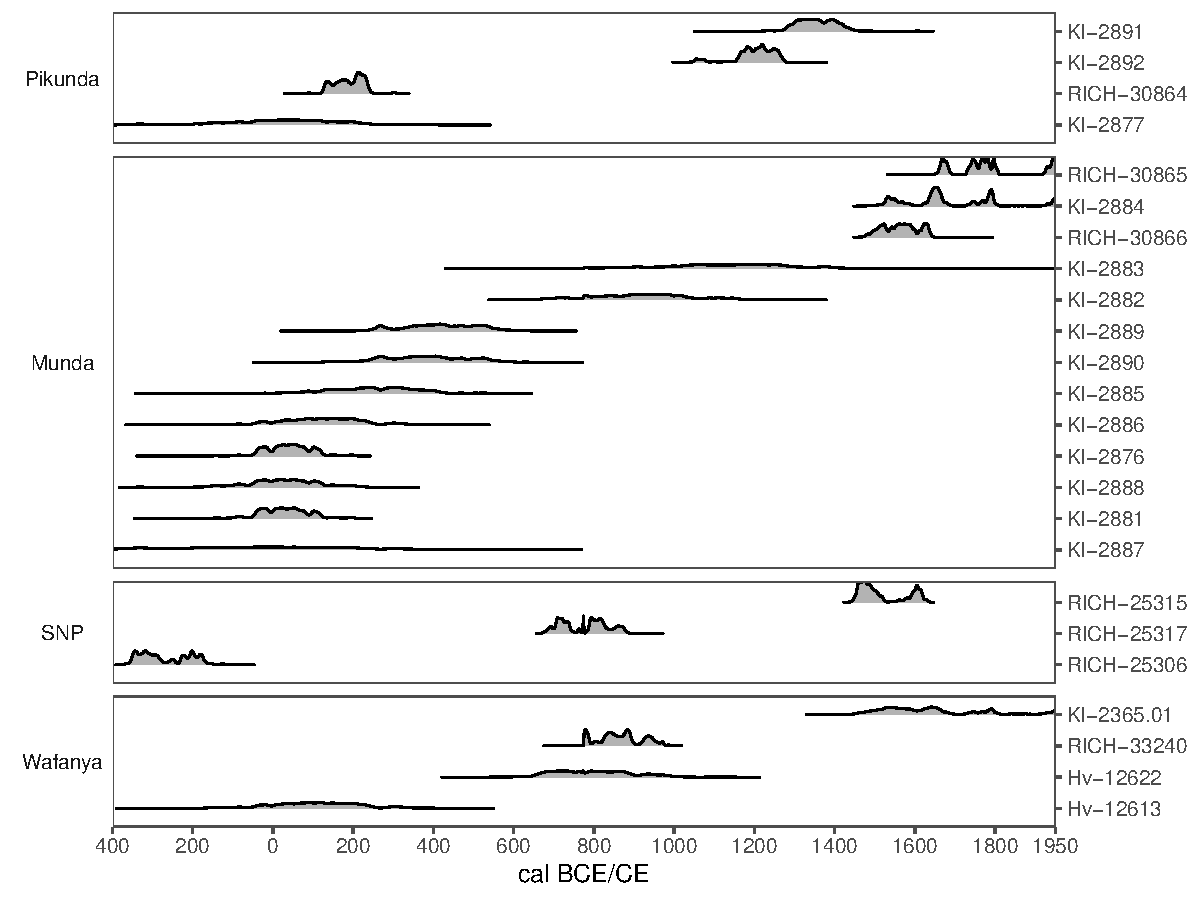
\includegraphics[width=\textwidth]{Fig_c14.pdf}
	\caption{Calibrated radiocarbon dates from the two case studies. Details see Tab.~\ref{tab:14C}.}
	\label{fig:c14}
\end{figure}

%\begin{figure}[H]
%	\centering
%	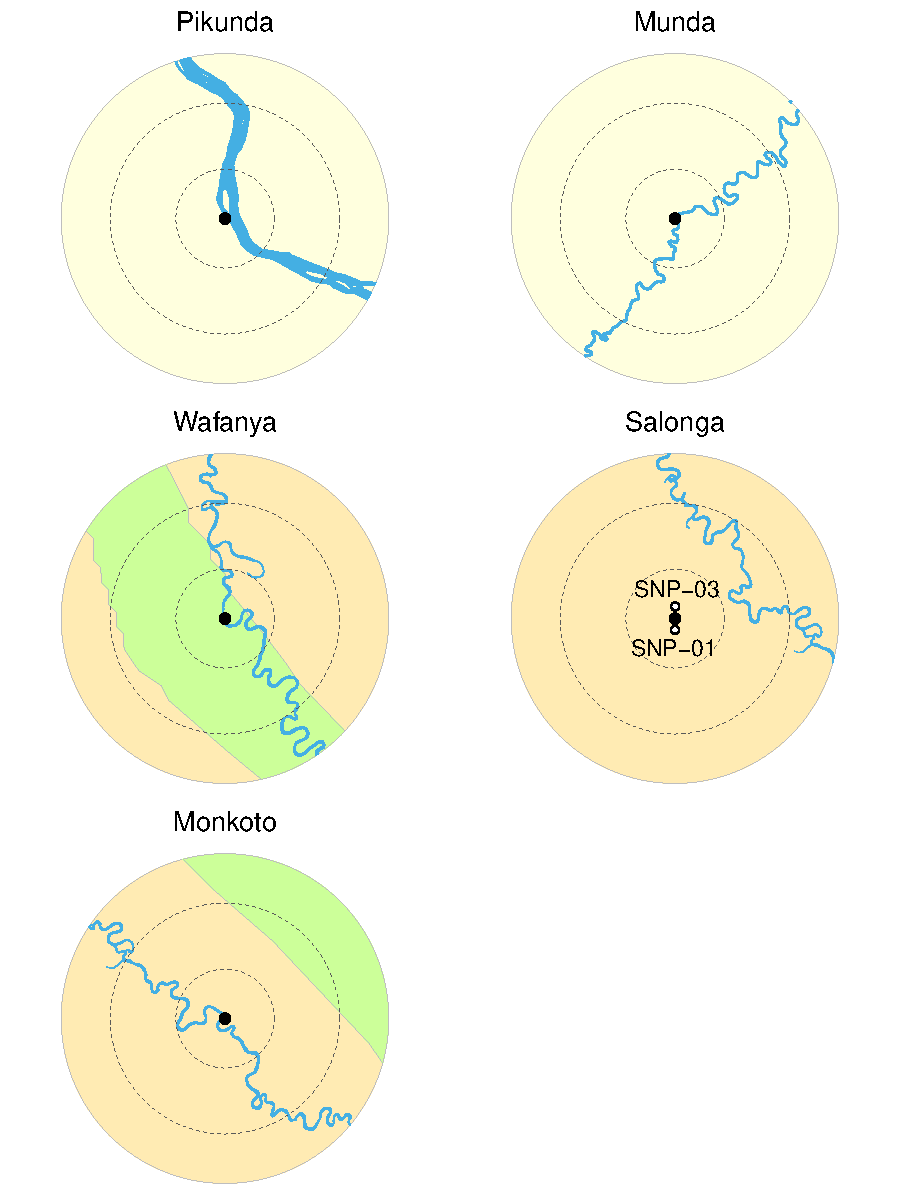
\includegraphics[width=\textwidth]{Fig_Map_Geol.pdf}
%	\caption{Local geological maps of the five sites (Fig.\ref{fig:map}) sampled for this study. Main geological units were derived from \citet{Persits.1997}. The circular cutouts correspond to Fig.~\ref{fig:map}B and show the main geological features 10~km from the site. The dashed circles indicate 3~km and 7~km distances from the sites, and represent reference values for how far potters travel to obtain their resources \citep{Whitbread.2001,Gosselain.2002,Gosselain.2005}.}
%	\label{fig:map.glg}
%\end{figure}

\begin{figure}[H]
	\begin{subfigure}[t]{\textwidth}
		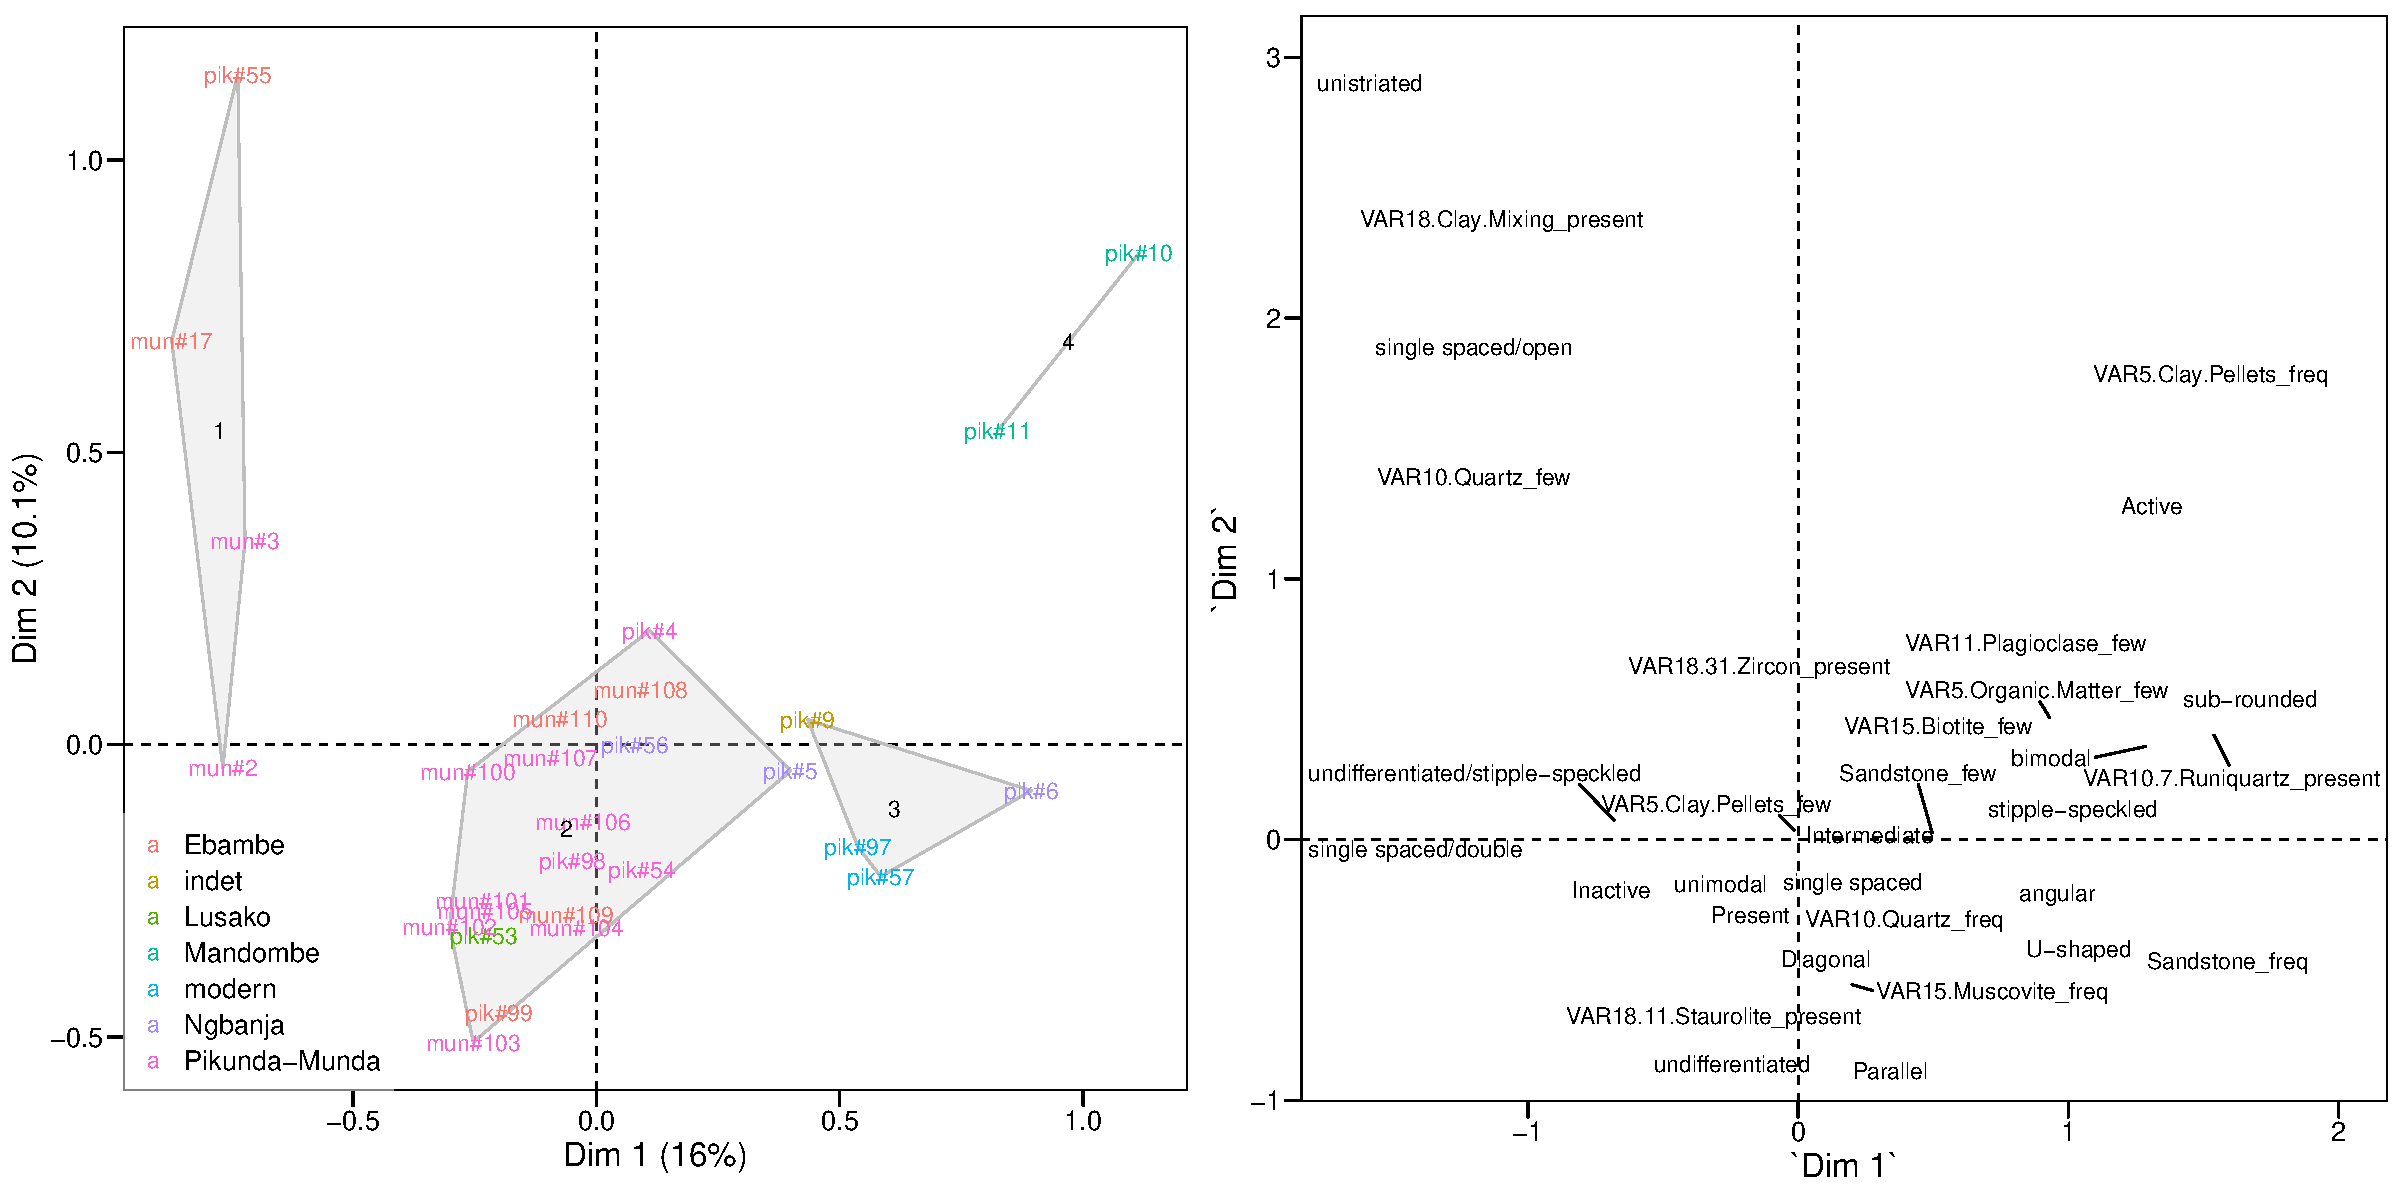
\includegraphics[width=\textwidth]{Fig_Petrofarbics_wCB.pdf}
		\caption{Case study I: Western Congo Basin}
		\label{fig:petrofrabrics.wCB}
	\end{subfigure}
	\begin{subfigure}[t]{\textwidth}
		\includegraphics[width=\textwidth]{Fig_Petrofarbics_luilaka.pdf}
		\caption{Case study II: Luilaka}
		\label{fig:petrofrabrics.luilaka}
	\end{subfigure}
	\caption{Score and loading plots of MCA from recorded petro-features used to differentiate qualitatively defined petrofrabrics \citep[cf.][]{Cau.2004}.}
	\label{fig:petrofrabrics}
\end{figure}

\begin{figure}[H]
	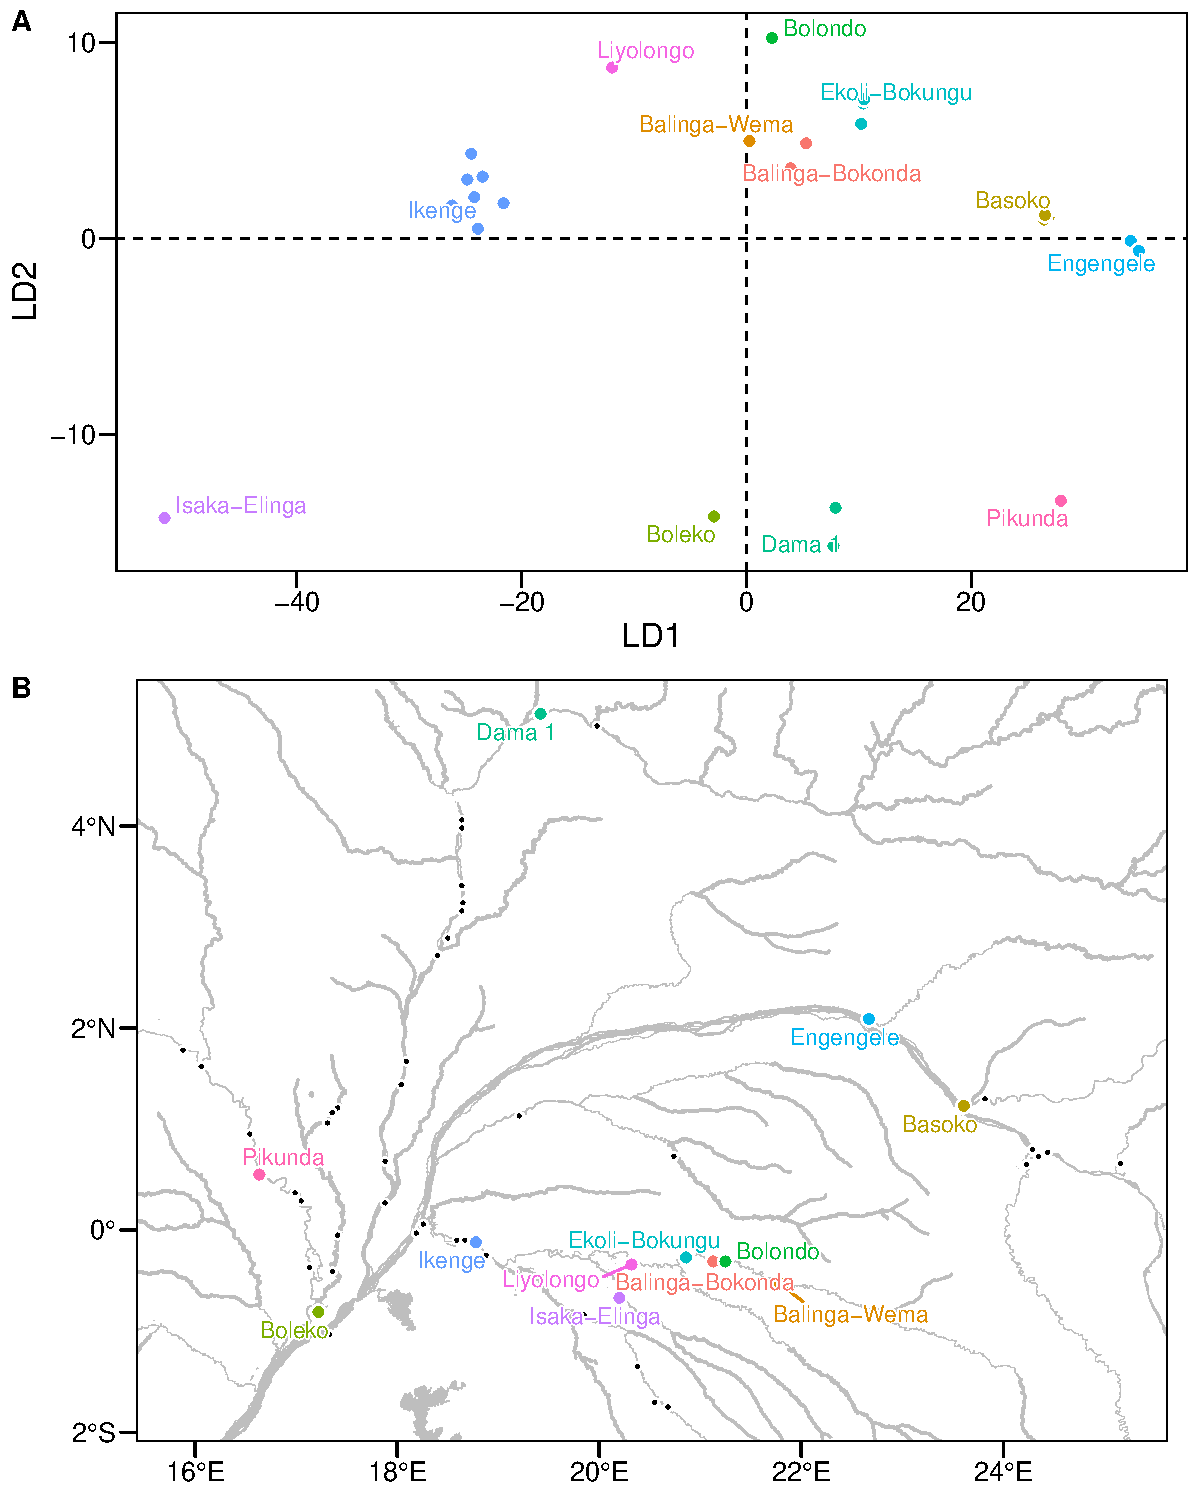
\includegraphics[width=\textwidth]{Fig_XRF_prov_LCA.pdf}
	\caption{A: Biplot of LDA on 25 samples with known provenance originating from 12 sites and map of sites (B; individually colored). The map (B) also shows all sites in the full XRF dataset (small black dots).}
	\label{fig:xrf.lda}
\end{figure}

\begin{figure}[H]
	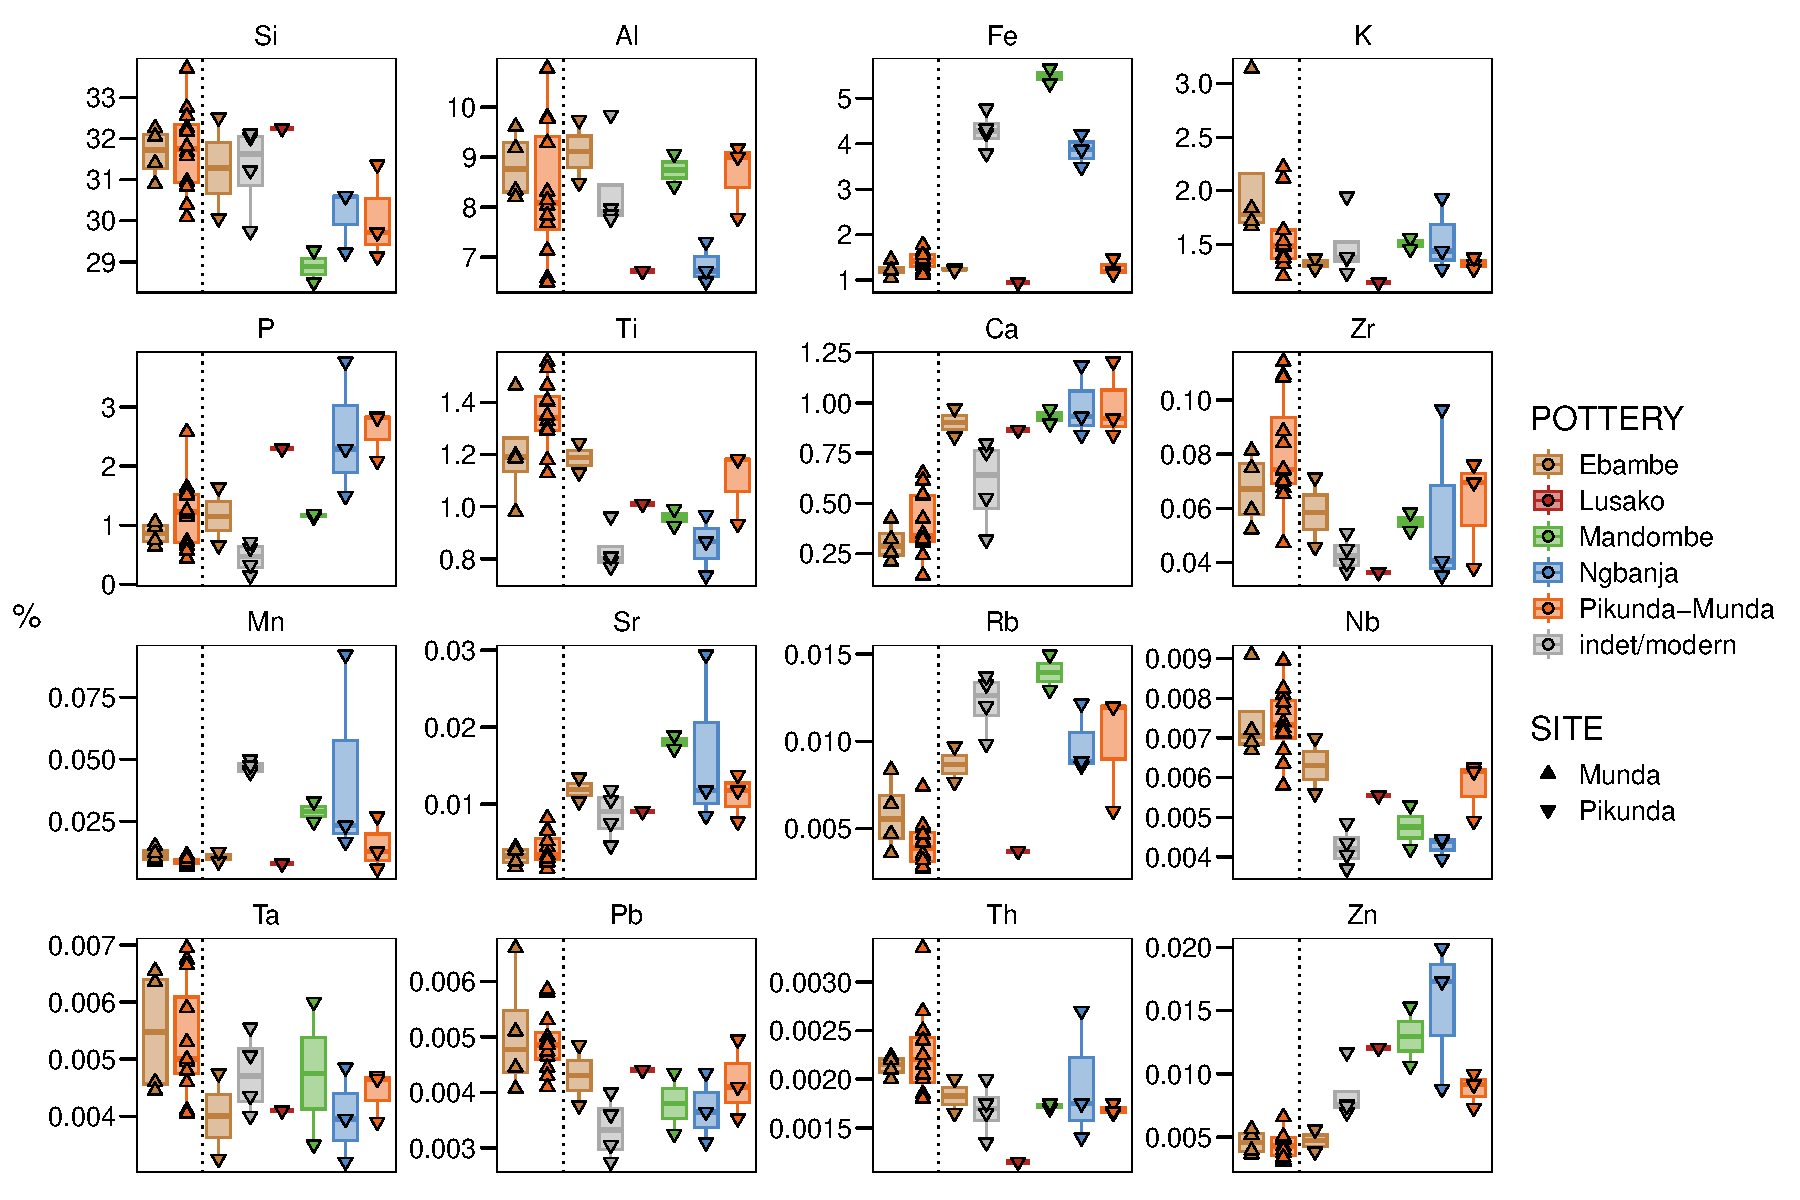
\includegraphics[width=\textwidth]{Fig_XRF_pik-mun.pdf}
	\caption{Elemental composition of samples from Pikunda and Munda, the two sites included in this study that are located in the Western Congo Basin. Colors represent distinct pottery styles shown in Figs.~\ref{fig:chrono}, \ref{fig:pik.pottery}, and \ref{fig:mun.pottery}.}
	\label{fig:xrf.pik-mun.comp}
\end{figure}

\begin{figure}[H]
	\centering
	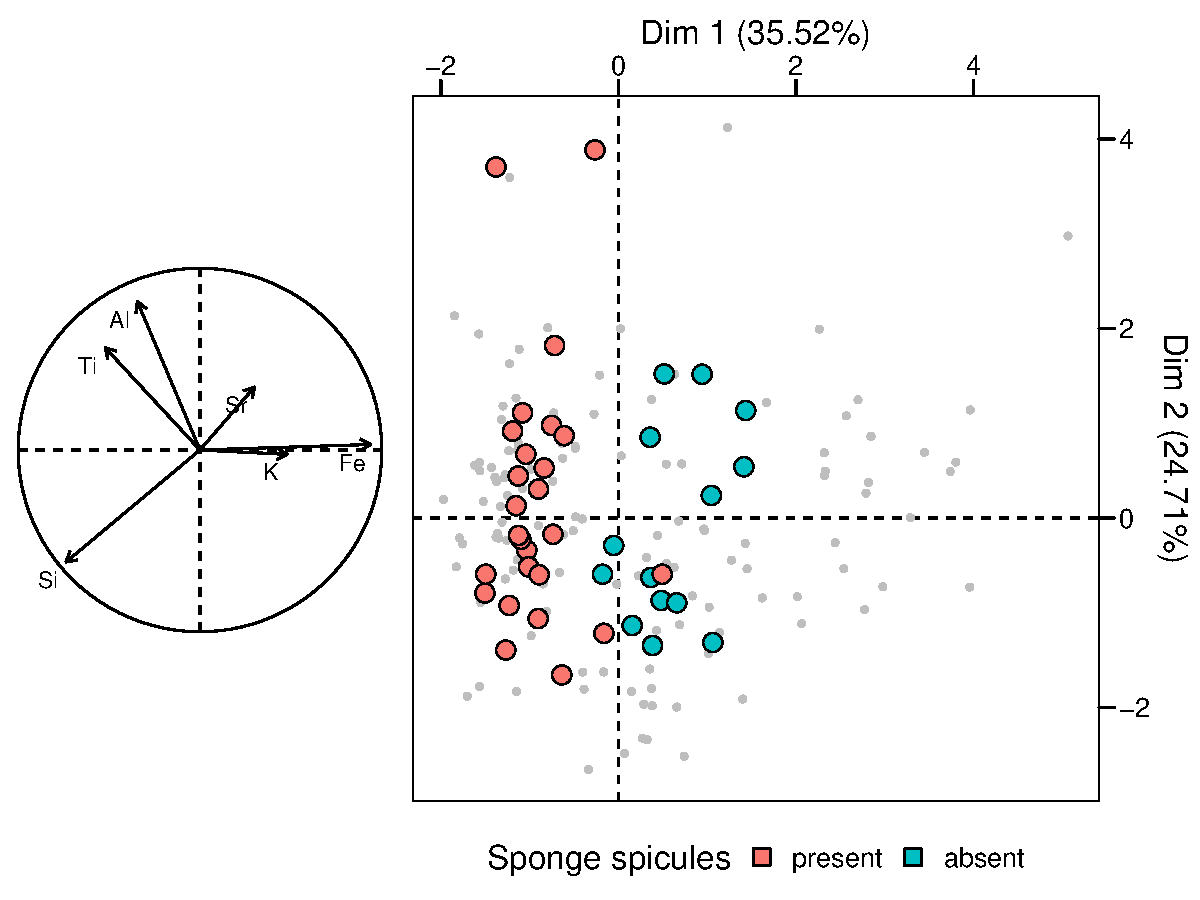
\includegraphics[width=.8\textwidth]{Fig_XRF_pca_clay_origin.pdf}
	\caption{Score and loading plots of PC 1 and 2 from the PCA's on the X-Ray intensities of six elements obtained from 169 ceramics sherds (grey dots). Highlighted are samples originating from the two case studies discussed in this paper. The coloration is derived of the sample containing sponge spicules or not. The presence of sponge spicules can be viewed as unambiguous evidence for the source clay procured by the pottery coming from a fluvial environment.}
	\label{fig:xrf.pca.clay.origins}
\end{figure}

\begin{figure}[H]
	\centering
	\begin{subfigure}[t]{.66\textwidth}
		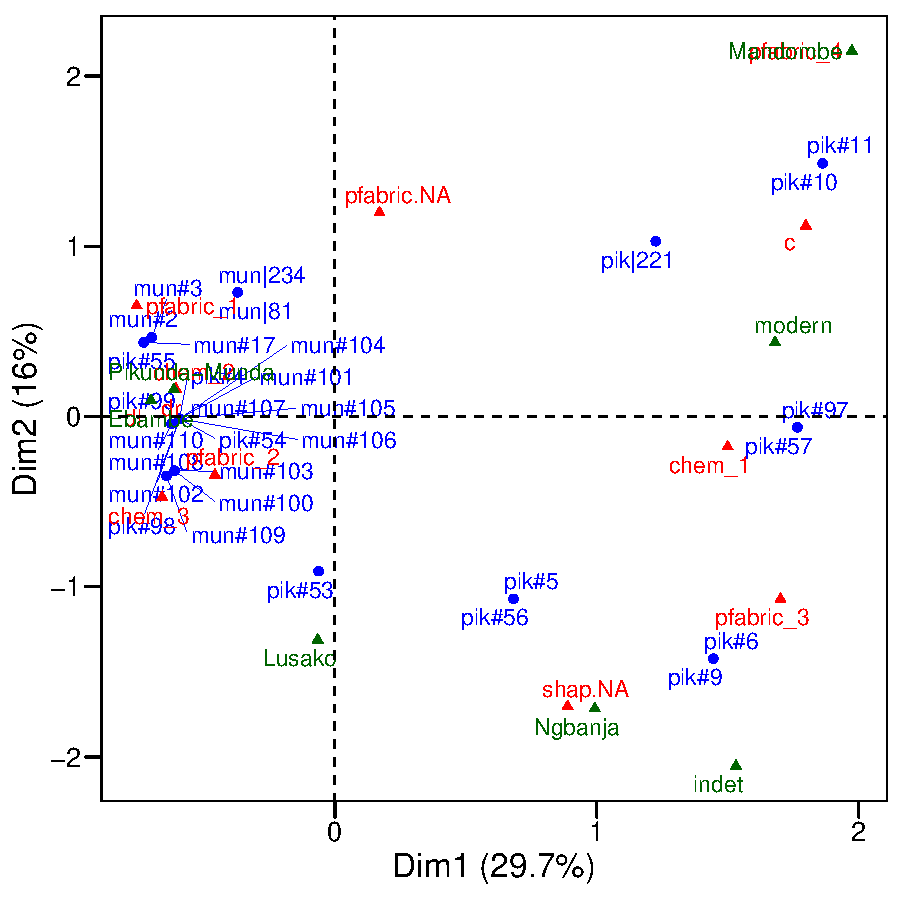
\includegraphics[width=\textwidth]{Fig_Synthesis_wCB.pdf}
		\caption{Case study I: Western Congo Basin\vspace{2em}}
		\label{fig:synthesis.wCB}
	\end{subfigure}
	\linebreak
	\begin{subfigure}[t]{.66\textwidth}
		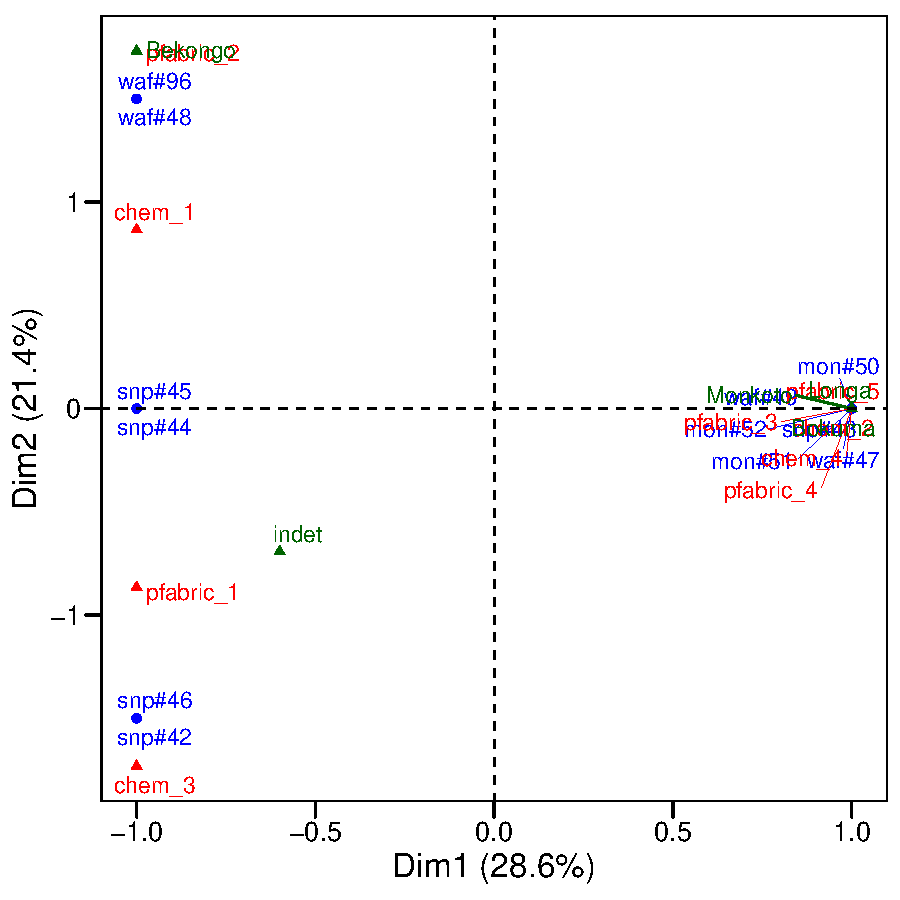
\includegraphics[width=\textwidth]{Fig_Synthesis_luilaka.pdf}
		\caption{Case study II: Luilaka}
		\label{fig:synthesis.luilaka}
	\end{subfigure}
	\caption{Score plots of MCA from sample (blue) based on the assigned petro-fabrics and grouping from XRF analysis (red) supplemented by the associated pottery style (green) highlighting the overall similarities and differences between the samples from the individual case studies.}
	\label{fig:synthesis}
\end{figure}

\begin{table*}[p]
	\begin{subtable}[t]{\textwidth}
		\centering
		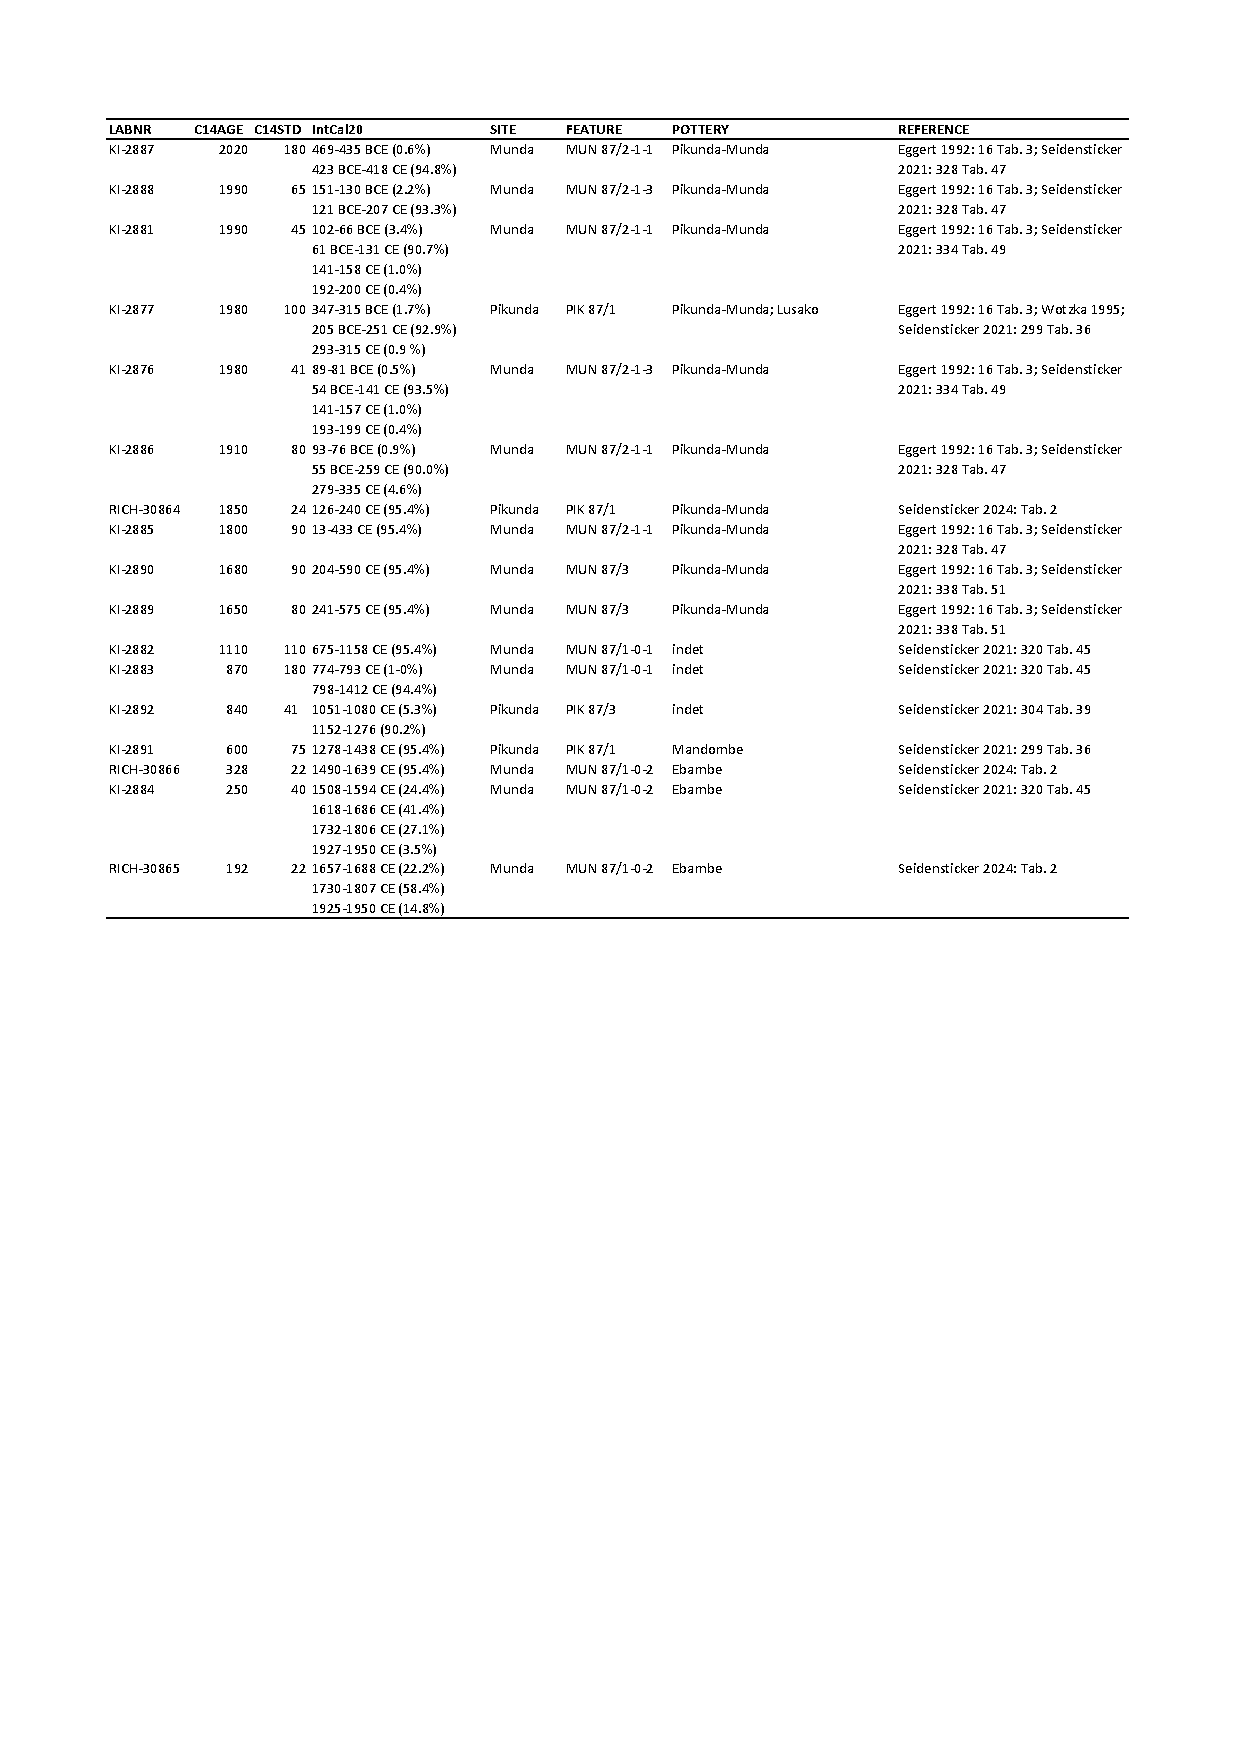
\includegraphics[width=\textwidth]{Tab_14C_nwCB.pdf}
		\caption{Case study I: Dates from Pikunda and Munda.}
		\label{tbl:c14_pik}
	\end{subtable}
	
	\begin{subtable}[t]{\textwidth}
		\centering
		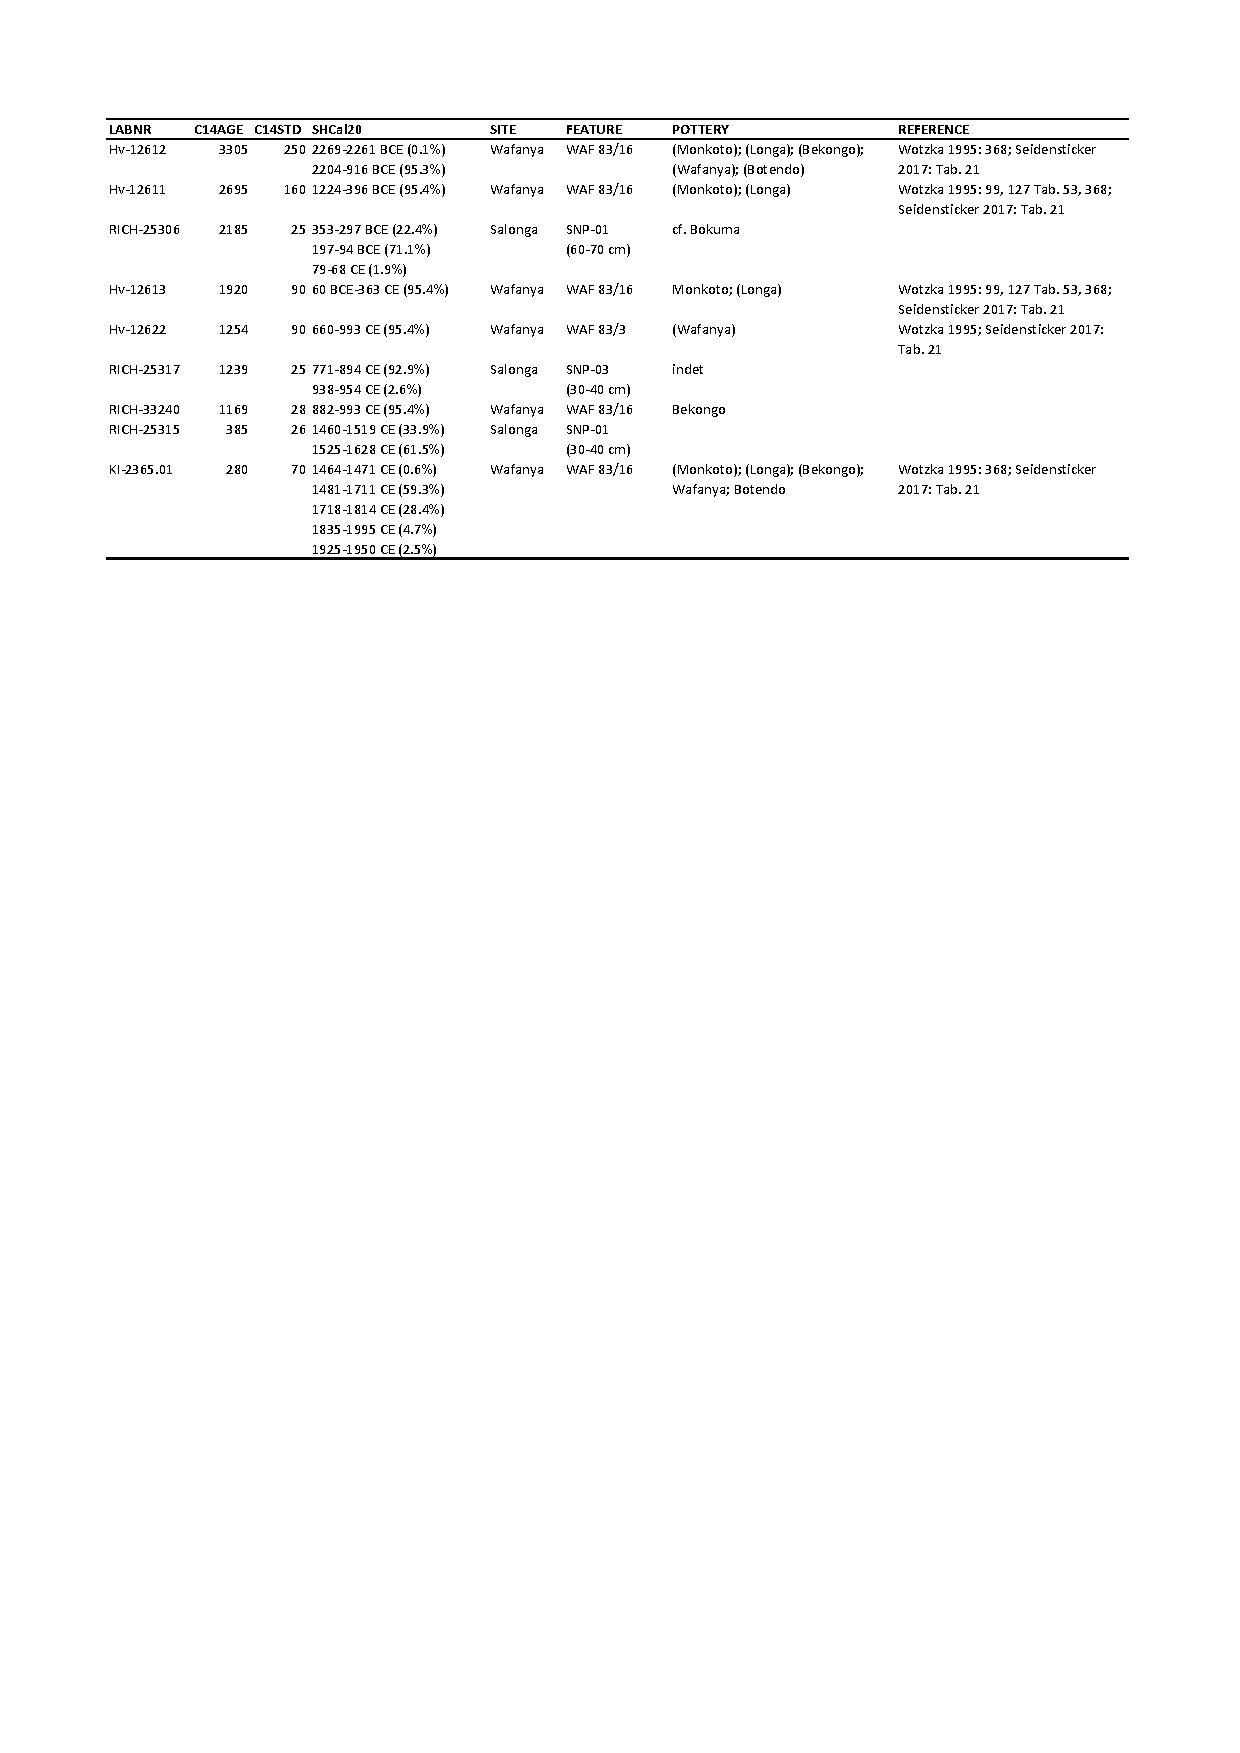
\includegraphics[width=\textwidth]{Tab_14C_ICB.pdf}
		\caption{Case study II: Dates from Monkoto and Wafanya. Note, the samples Hv-12611 \& Hv-12612 are considered not representative for the archaeological feature and finds they were associated with by \citet[99, 127 Tab.~53, 368]{Wotzka.1995} and are viewed as potential lab errors, following \citet{Geyh.1990}.}
		\label{tbl:c14_slg}
	\end{subtable}
	
	\caption{Calibrated ages of radiocarbondates from the two case studies (cf. Fig.~\ref{fig:c14}). A comprehensive record of all published radiocarbon dates in Central Africa can be found in the online aDRAC repository \cite{Seidensticker.2021f}. Entries in the pottery field marked in parentheses indicate that sherds of this style were found in association with the sample, but that the date was not regarded as representative for this pottery \citep[193--204]{Wotzka.1995, Seidensticker.2021e}, potentially due to lab-errors \citep{Geyh.1990}.}
	\label{tab:14C}	
\end{table*}

\newpage
\bibliographystyle{elsarticle-harv}
\bibliography{bib.bib}

\end{document}
